\graphicspath{{}{miniboone/figs/}{miniboone/}{Diagrams/}}

Anomalies in short-baseline accelerator and reactor experiments~\cite{Athanassopoulos:1996jb,Aguilar:2001ty,AguilarArevalo:2007it,Aguilar-Arevalo:2018gpe} are yet to have satisfying explanations. Minimal extensions of the three-neutrino framework to explain the anomalies introduce the so-called sterile neutrino states, which do not participate in Standard Model (SM) interactions in order to agree with measurements of the Z-boson invisible decay width~\cite{ALEPH:2010aa}. Unfortunately, these minimal scenarios are disfavoured as they fail to explain all data~\cite{Collin:2016aqd, Capozzi:2016vac, Dentler:2018sju}. This has led the community to explore non-minimal scenarios. Along this direction, we have already study a well-motivated neutrino-mass model that can also explain the short-baseline anomalies in Chapter 5. In this chapter, we will focus on the phenomenological realisations of dark neutrinos that have been proposed as an explanation of the anomalous observation of $\nu_e$-like events in MiniBooNE~\cite{Aguilar-Arevalo:2018gpe}.

MiniBooNE is a mineral oil Cherenkov detector located in the Booster Neutrino Beam (BNB), at Fermilab~\cite{AguilarArevalo:2008yp,AguilarArevalo:2008qa}. From data collected between 2002 to 2017, the experiment has observed an excess of $\nu_e$-like events that is currently in tension with the standard three-neutrino prediction at a level of $4.7 \sigma$~\cite{Aguilar-Arevalo:2018gpe}. While it is possible that the excess is fully or partially due to systematic uncertainties or SM backgrounds~(see, \textit{e.g.},~\cite{AguilarArevalo:2008rc,Aguilar-Arevalo:2012fmn,Hill:2010zy}), many Beyond the Standard Model (BSM) explanations have been put forth. These new physics (NP) scenarios typically require the existence of new particles, which can: participate in short-baseline oscillations~\cite{Murayama:2000hm,Strumia:2002fw,Barenboim:2002ah, GonzalezGarcia:2003jq,Barger:2003xm,Sorel:2003hf,Barenboim:2004wu, Zurek:2004vd, Kaplan:2004dq, Pas:2005rb,deGouvea:2006qd,Schwetz:2007cd, Farzan:2008zv,Hollenberg:2009ws,Nelson:2010hz,Akhmedov:2010vy, Diaz:2010ft,Bai:2015ztj, Giunti:2015mwa,Papoulias:2016edm, Moss:2017pur,Carena:2017qhd}, change the neutrino propagation in matter~\cite{Liao:2016reh, Liao:2018mbg,Asaadi:2017bhx,Doring:2018cob}, be produced in the beam or in the detector and its surroundings~\cite{Gninenko:2009ks,Gninenko:2010pr,Dib:2011jh,McKeen:2010rx,Masip:2012ke, Masip:2011qb,Gninenko:2012rw,Magill:2018jla}. These models either increase the conversion of muon- to electron-neutrinos or produce electron-neutrino-like signatures in the detector, where in the latter category one typically exploits the fact that the LSND and MiniBooNE are Cherenkov detectors that cannot distinguish between electrons and photons. Although it is possible to consider MiniBooNE explanations that have little to no theoretical motivation, recent models~\cite{Bertuzzo:2018itn,Bertuzzo:2018ftf,Ballett:2018ynz} are motivated by neutrino-mass generation via hidden interactions in the heavy neutrino sector. In particular, the common feature of these models is the upscattering into a heavy neutrino, usually with tens to hundreds of MeV in mass, which subsequently decays into a pair of electrons. If collimated, this pair of electrons can fake a single-electron signature. 

Our main contributin is introducing new techniques to probe models that rely on the ambiguity between photons and electrons to explain the MiniBooNE observation, using the dark neutrino model from~\cite{Bertuzzo:2018itn,Bertuzzo:2018ftf} as a benchmark scenario. 
Our analysis relies on neutrino-electron scattering measurements~\cite{Auerbach:2001wg,Deniz:2009mu,Bellini:2011rx,Park:2013dax,Valencia:2019mkf,Park:2015eqa,Valencia-Rodriguez:2016vkf,DeWinter:1989zg,Geiregat:1992zv,Vilain:1994qy}. This process is currently used to normalize the neutrino fluxes, due to its well-understood cross section, and has been a fertile ground for light NP searches~\cite{Pospelov:2017kep,Lindner:2018kjo,Magill:2018tbb}. Here, however, we expand the capability of these measurements to probe BSM-produced photon-like signatures, by developing a new analysis using previously neglected sideband data. Our technique is complementary to recent searches for coherent single-photon topologies~\cite{Abe:2019cer}.
Since the upscattering process has a threshold of tens to hundreds of MeV, we focus on two high-energy neutrino experiments: \minerva~\cite{Park:2013dax,Valencia:2019mkf,Park:2015eqa,Valencia-Rodriguez:2016vkf}, a scintillator detector in the Neutrinos at the Main Injector (NuMI) beamline at Fermilab, and CHARM-II~\cite{DeWinter:1989zg,Geiregat:1992zv,Vilain:1994qy}, a segmented calorimeter detector at CERN along the Super Proton Synchrotron (SPS) beamline. These experiments are complementary in the range of neutrino energies they cover and have different background composition. In all cases a relevant sideband measurement exists, allowing us to take advantage of the excellent particle reconstruction capabilities of \minerva and the precise measurements at CHARM-II to constrain NP.
%

\section{Dark Neutrinos at MiniBooNE}

%%% DIAGRAM %%%
\begin{figure}[t!]
    \centering
    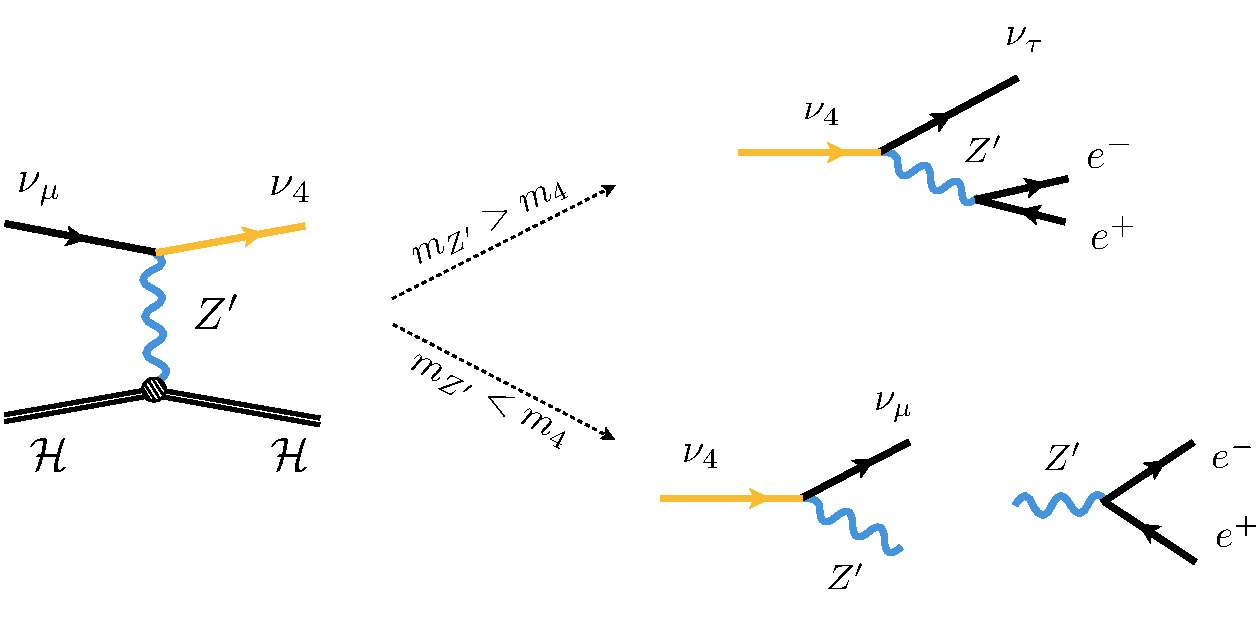
\includegraphics[width=0.9\textwidth]{Dark_neutrinos.pdf}
    \caption[Dark neutrino signal at MiniBooNE.]{The dark neutrino signal at MiniBooNE. We show the two phenomenological realisations of the dark neutrino model with a heavy (top) and light (bottom) mediator. In the heavy case, large $|U_{\tau4}|^2$ is required to shorten the $\nu_4$ lifetime.\label{fig:diagram}}
\end{figure}
%%%%%%%%%%%%%%%%%%%%%%%%%
 We limit our discussion to the minimal version of the model that could explain the MiniBooNE excess. This contains at least one Dirac heavy neutrino\footnote{Models with the decay of Majorana particles will lead to greater tension with the angular distribution at MiniBooNE due to their isotropic nature~\cite{Formaggio:1998zn,Balantekin:2018ukw}.}, $\nu_D$, charged under a new U$(1)^\prime$ gauge group, which is part of the particle content and gauge structure needed for mass generation. The dark sector is connected to the SM in two ways: through kinetic mixing between the new gauge boson and hypercharge, and through neutrino mass mixing. We start by specifying the kinetic part of the NP Lagrangian
%
\begin{equation}
\mathscr{L}_{\rm kin} \supset
\;\; \frac{1}{4} \hat{Z}^{\prime}_{\mu \nu} \hat{Z}^{\prime \mu \nu} + \frac{\sin{\chi}}{2} \hat{Z}^{\prime}_{\mu \nu} \hat{B}^{\mu \nu} + \frac{m_{\hat{Z}^\prime}^2}{2} \hat{Z}^{\prime \mu} \hat{Z}^\prime_{\mu},
\end{equation}
%
where $\hat{Z}^{\prime \mu}$ stands for the new gauge boson field, $\hat{Z}^{\prime \mu\nu}$ its field strength, and $\hat{B}^{\mu \nu}$ the hypercharge field strength. After usual field redefinitions~\cite{Chun:2010ve}, we arrive at the physical states of the theory. Working at leading order in $\chi$ and assuming $m_{Z^\prime}^2/m_{Z}^2$ to be small, we can specify the relevant interaction Lagrangian as
%
\begin{equation}
\mathscr{L}_{\rm int} \supset \;\;g_D \overline{\nu}_D \gamma_\mu \nu_D Z^{\prime \mu}
 + e \varepsilon Z'^{\mu}J^{\rm EM}_{\mu},
\end{equation}
%
where $J^{\rm EM}_{\mu}$ is the SM electromagnetic current, $g_D$ is the U$(1)^\prime$ gauge coupling assumed to be $\mathcal{O}(1)$, and $\varepsilon \equiv c_{\rm w} \chi$, with $c_{\rm w}$ being the cosine of the weak angle. Additional terms would be present at higher orders in $\chi$ and mass mixing with the SM $Z$ is also possible, though severely constrained. 
After electroweak symmetry breaking, the dark neutrino $\nu_D$ is a superposition of neutrino mass states. The flavor and mass eigenstates are related via 
\begin{equation}
    \nu_\alpha = \sum^{4}_{i=1} U_{\alpha i}\nu_{i}, \quad (\alpha=e,\mu,\tau,D),
\end{equation}
where $U$ is a $4\times4$ unitary matrix. It is expected that $|U_{\alpha 4}|$ is small for $\alpha = e, \mu, \tau$, but $|U_{D4}|$ can be of $\mathcal{O}(1)$~\cite{Parke:2015goa,Collin:2016aqd}. The choice of $m_4$ and $m_{Z^\prime}$ has important consequences for the allowed decays of the new particle content. We focus on the case in which $m_4 > m_{Z^\prime}$, where the two body $\nu_4 \to \nu_\alpha Z^\prime$ decay is allowed. In addition, the mass of the new gauge boson is kept below $\sim100$ MeV, making the decay into $e^+e^-$ pairs the dominant channel. Decay into a pair of neutrinos is possible, but is subdominant provided neutrino mixing is small. 
%%

\subsection{Signature and region of interest}

The heavy neutrino is produced from an active flavour state upscattering on a nuclear target $A$, $\nu_\alpha A \to \nu_4 A$. The upscattering cross section is proportional to $\alpha_D \alpha_\textsc{qed}\varepsilon^2 |U_{\alpha 4}|^2$, dominated by $|U_{\mu 4}|$ since all current accelerator neutrino beams are composed mainly of muon neutrinos. This production can happen off the whole nucleus in a coherent way or off individual nucleons. For $m_{Z^\prime} \lesssim 100$ MeV, the production will be mainly coherent, but for heavier masses, such as the ones considered in~\cite{Ballett:2018ynz}, incoherent upscattering dominates. In Fig.~\ref{fig:cross_section}, we show the NP cross section at the benchmark point of~\cite{Bertuzzo:2018itn} and compare it with the quasi-elastic cross section. By superimposing the cross section on the neutrino fluxes of \minerva and MiniBooNE, we make it explicit that the larger energies at \minerva and CHARM-II are ideal to produce $\nu_4$. Once produced, $\nu_4$ predominantly decays into a neutrino and a dielectron pair, $\nu_4 \to \nu_\alpha e^+ e^-$, either via an on-shell~\cite{Bertuzzo:2018itn} or off-shell~\cite{Ballett:2018ynz} $Z^\prime$ depending on the choice of $m_4$ and $m_{Z^\prime}$. In this work, we restrict our discussion to the $m_4 > m_{Z^\prime}$ case, where the upscattering is mainly coherent and is followed by a chain of prompt two body decays $\nu_4 \to \nu_\alpha (Z^\prime \to e^+ e^-)$. The on-shell $Z^\prime$ is required to decay into an overlapping $e^+e^-$ pair, setting a lower bound on its mass of a few MeV. Experimentally, however, $m_{Z^\prime} > 10$ MeV for $e \epsilon \sim 10^{-4}$ to avoid beam dump constraints~\cite{Bauer:2018onh}.
Increasing $m_{Z^\prime}$ increases the ratio of incoherent to coherent events, and makes the electron pair less overlapping.
Even though we focus on overlapping $e^+e^-$ pairs, we note that a significant fraction of events would appear as well-separated showers or as a pair of showers with large energy asymmetry, similarly to neutral current (NC) $\pi^0$ events. The asymmetric events also contribute to the MiniBooNE excess and offer a different target for searches in $\nu-e$ scattering data.

A fit to the neutrino energy spectrum at MiniBooNE was performed in ~\cite{Bertuzzo:2018itn} and is reproduced in~\reffig{fig:final_plot}. We have performed our own fit to the MiniBooNE energy spectrum using the data release from~\cite{Aguilar-Arevalo:2018gpe}, and our results agree with~\cite{Bertuzzo:2018itn}. This fit leads to preferred values of $m_4$ close to 100 MeV and $|U_{\mu 4 }| \sim 10^{-4}$. Unfortunately, this energy-only fit neglects the distribution of the excess events as a function of their angle $\theta$ with respect to the beam.
This is important, as the total observed excess contains only $\approx 50\%$ of the events in the most forward bin ($0.8 < \cos{\theta} < 1.0$), with a statistical uncorrelated uncertainty of 5\% on this quantity.  
 
As was recently pointed out in~\cite{Jordan:2018qiy}, few NP scenarios can reproduce the angular distribution of the MiniBooNE excess. Among these are models where new unstable particles are produced in inelastic collisions in the detector, such as the present case.
Here, large $\theta$ can be achieved by tweaking the mass of the heavy neutrino; the signal becomes less forward as $\nu_4$ becomes heavier.
To show this, we use our dedicated Monte Carlo (MC) simulation to asses the values of $m_4$ preferred by MiniBooNE data~\footnote{Since the released MiniBooNE data do not provide the correlation between angle and energy, and their associated systematics, an energy-angle fit is not possible.}. For $m_{Z^\prime} = 30$ MeV and $m_4 = 100$, $200$, and $400$ MeV, we find that 98\%, 87\%, and 70\% of the NP events would lie in the most forward bin, respectively. 
The latter, as expected, is close to the benchmark point of~\cite{Bertuzzo:2018itn}. Thus the relevant region for the MiniBooNE angular distribution is $m_4 \gtrsim 400$ MeV for $m_{Z^\prime} = 30$ MeV.
 
\section{Dark Neutrinos in Neutrino-Electron Scattering}
%%%%%%%%%%%%% Cross Section %%%
\begin{figure}[t!]
    \centering
    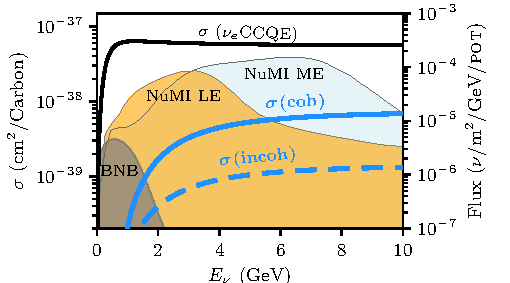
\includegraphics[width=0.65\textwidth]{cross_sections.pdf}
%     \caption[Upscattering total cross section.]{The quasi-elastic cross section for $6p^+$ is shown as a function of the neutrino energy (solid black line). Similarly the coherent, out of a carbon atom, and the diffractive NP contributions for the benchmark point of~\cite{Bertuzzo:2018itn} are shown as solid and dashed blue lines, respectively. In the background, the light gray shaded region is the Booster Neutrino Beam (BNB) flux shape, while the light golden region is the Neutrinos at the Main Injector (NuMI) low-energy neutrino-mode flux.}{\label{fig:cross_section}}
    \caption[Upscattering total cross section.]{The quasi-elastic cross section on Carbon ($6p^+$) is shown as a function of the neutrino energy (solid black line). The coherent (solid blue) and incoherent (dashed blue) scattering NP cross sections are also shown for the benchmark point of~\cite{Bertuzzo:2018itn}. In the background, we show the BNB flux of $\nu_\mu$ at MiniBooNE (light gray), and the NuMI beam neutrino flux at MINER$\nu$A for the LE (light golden) and ME (light blue) runs in neutrino mode.\label{fig:cross_section}}
\end{figure}
%%%%%%%%%%%%%%%%%%%%%%%%%%%%%%%%%%%%%%%%%%%%%%%%%%

Our goal is to develop new techniques to probe dark neutrino models in neutrino-electron scattering measurements. Our analysis showcases a generic way to look for models that rely on the ambiguity between photons and electrons to explain the MiniBooNE observation. Due to the electron-like nature of the excess, neutrino-electron scattering measurements~\cite{Auerbach:2001wg, Deniz:2009mu,Bellini:2011rx,Park:2013dax,Vilain:1994qy} provide the kind of signature one would look for. Although these measurements have been shown to provide powerful constraints on light NP~\cite{Pospelov:2017kep,Lindner:2018kjo,Magill:2018tbb}, the unique photon-like topology of the signatures we consider requires us to go beyond the final processed sample quoted by the experiments and make use of sideband measurements to constrain them.
Since the typical heavy neutrino mass is in the hundreds-of-MeV regime, we focus on two high-energy neutrino experiments: \minerva~\cite{Park:2013dax,Park:2015eqa,Valencia-Rodriguez:2016vkf} and CHARM-II~\cite{DeWinter:1989zg,Geiregat:1992zv,Vilain:1994qy}. These experiments are complementary in neutrino energy and background composition. In both cases we make use of sideband measurements, taking advantage of the excellent particle reconstruction capabilities of \minerva and the precise measurements at CHARM-II to constrain NP. In Fig.~\ref{fig:cross_section}, we show the cross section at the benchmark point of~\cite{Bertuzzo:2018ftf} and compare it with the quasi-elastic cross section. By superimposing the cross section on the neutrino fluxes of \minerva and MiniBooNE, we make it explicit that the larger energies at \minerva and CHARM-II are ideal to probe these models. 


\section{Simulation Details}
%
\begin{figure}[t]
 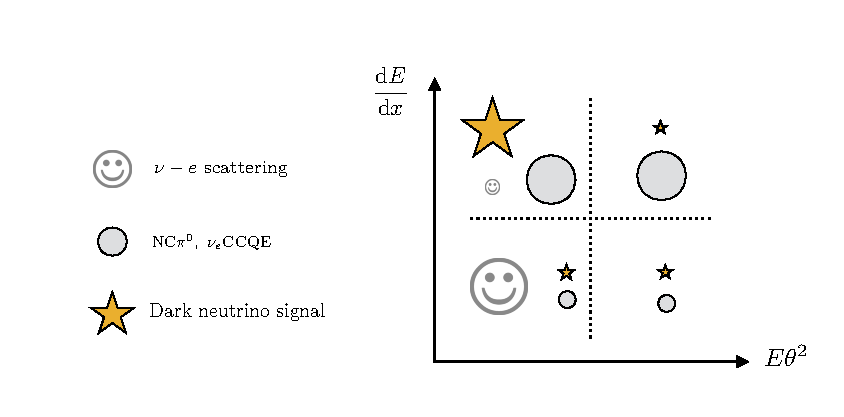
\includegraphics[width = 0.9\textwidth]{MiniBooNE_tests.pdf}
 \caption[Diagram of the sidebands in neutrino-electron scattering analyses.]{A schematic representation of the relative number of events in sideband regions of neutrino-electron scattering analyses.}
\end{figure}
%
We generate events distributed according to the upscattering cross section for the process $\nu_\mu A \to \nu_4 A$, where $A$ is a nuclear target. Here, we only discuss upscattering on nuclei, as the number of elastic scattering on protons is much smaller at these $Z^\prime$ masses (see \reffig{fig:cross_section}). We then implement the chain of two-body decays: $\nu_4 \to \nu_\mu Z^\prime$ followed by $Z^\prime \to e^+ e^-$. To go from our MC output to the predicted experimental signature, we perform three procedures. First, we smear the energy and angles of the $e^+$ and $e^-$ originating from the decay of the $Z^\prime$ according to detector dependent Gaussian energy and angular resolutions. Next, we select all events with an overlapping $e^+e^-$ pair, which is assumed to be reconstructed as a single electromagnetic (EM) shower. This guarantees that the events behave like a photon shower inside the detector~\footnote{For MiniBooNE, we also include events that are highly asymmetric in energy, \textit{i.e.}, $E_{\pm} > 30$ MeV and $E_{\mp} < 30$ MeV, where the most energetic shower defines the angle with respect to the beam.)}. Finally, for \minerva and CHARM-II, these samples are subject to analysis-dependent kinematical cuts to determine if they contribute to the $\nu-e$ scattering sample. Detector resolutions, requirements for the dielectron pair to be overlapping, and analysis-dependent cuts are summarized in \reftab{tab:parameters}. We now list the experimental parameters used in our simulations for each individual detector. 
%% DIAGRAM %%%
% \begin{figure}[t]
%     \centering
%     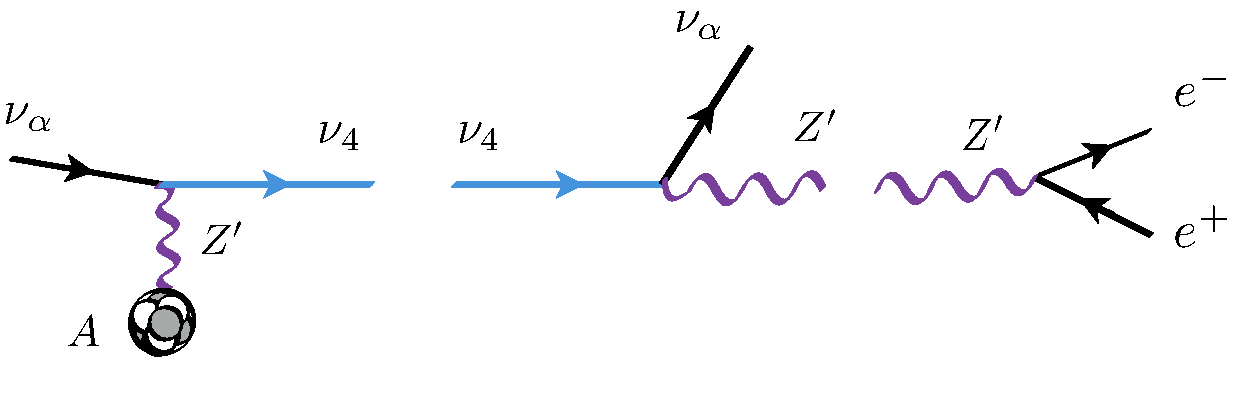
\includegraphics[width=0.49\textwidth]{diagram.pdf}
%     \caption{{\textit{Illustration of heavy neutrino production.}} Left: production of the heavy mass state via upscattering. Center: Decay of the heavy neutrino into a light neutrino and a gauge boson. Right: Decay of a gauge boson into a pair of electrons that produce the experimental signature.\label{fig:diagram}}
% \end{figure}

\paragraph{CHARM-II} The CHARM-II experiment is simulated using the CERN West Area Neutrino Facility (WANF) wide band beam ~\cite{Vilain:1998uw}. The total number of POT is $2.5 \times 10^{19}$ for the $\nu$ and $\overline{\nu}$ run combined. We assume glass to be the main detector material (SiO$_2$), such that we can treat neutrino scattering off an average target with $\langle Z\rangle=11$ and $\langle A \rangle = 20.7$~\cite{DeWinter:1989zg,Vilain:1993sf}. The fiducial volume in our analysis is confined to a transverse area of $320$cm$^2$ (corresponding to a fiducial mass of $547$t) and the detection efficiency is taken to be $76\%$ (efficiency for $\pi^0$ sample is quoted at $82\%$~\cite{Vilain:1992wx}). We reproduce the total number of $\nu-e$ scattering events with $3$ GeV $< E_{\rm vis} <24$ GeV, namely $2677+2752$, to within a few percent level when setting the number of POTs in $\nu$ mode to be $1.69$ of that in the $\overline{\nu}$ mode~\cite{Geiregat:1991md}. We assume a flux uncertainty of $\sigma_\alpha = 4.7\%$ for neutrino, and $\sigma_\alpha = 5.2\%$ for antineutrino beam~\cite{Vilain:1992wx}. The background uncertainty is constrained to be $\sigma_\beta = 3\%$ using the data with $E_{\rm vis} \theta^2 > 30$ MeV, where the number of new physics events is negligible.

\paragraph{MINER$\nu$A} For our MINER$\nu$A simulation, we use the LE and ME NuMI neutrino fluxes~\cite{AliagaSoplin:2016shs}. The total number of POT is $3.43\times 10^{20}$ for LE data, and $11.6\times10^{20}$ for ME data. The detector is assumed to be made of CH, with a fiducial mass of $6.10$t and detection efficiencies of $73\%$~\cite{Parke:2015goa,Valencia:2019mkf}. We assume a flux uncertainty of $\sigma_\alpha = 10\%$ for both the LE and ME modes~\cite{Aliaga:2016oaz}. Due to the tuning performed in the sideband of interest, the uncertainties on the background rate are much larger. For the LE, we take $\sigma_\beta = 30\%$, while for the ME data  $\sigma_\beta = 50\%$. Although tuning is significant for the coherent $\pi^0$ production sample, the overall rate of backgrounds in the sideband with large $dE/dx$ does not vary by more than $20\%$ ($40\%$) in the LE (ME) tuning.  

\paragraph{MiniBooNE} To simulate MiniBooNE, we use the Booster Neutrino Beam (BNB) fluxes from Ref.~\cite{AguilarArevalo:2008yp}. Here, we only discuss the neutrino run, although the predictions for the antineutrino run are very similar. We assume a total of $12.84 \times 10^{20}$ POT in neutrino mode. The fiducial mass of the detector is taken as $450$t of CH$_2$. In order to apply detector efficiencies, we compute the reconstructed neutrino energy under the assumption of CCQE scattering
\begin{align}
 E_\nu^{CCQE} = \frac{E_{\rm vis} m_p}{m_p - E_{\rm vis} (1 - \cos{\theta}) },
\end{align}
where $E_{\rm vis} = E_{e^+} + E_{e^-}$ is the total visible energy after smearing. Under this assumption, we can apply the efficiencies provided by the MiniBooNE collaboration~\cite{Aguilar-Arevalo:2012fmn}.

\renewcommand{\arraystretch}{1.2}
\begin{table*}[t]
    \centering
    \begin{tabular}{|lp{5.2cm}p{2.8cm}p{3cm}|}
        \hline       
        Experiment & Detector Resolution&Overlapping & Analysis Cuts  \\
        \hline        \hline
        MiniBooNE & & & \\\hline
         & $\sigma_E/E = 12\%$ \newline $\sigma_\theta = 4{^\circ}$ & $E_{+} > 30$ MeV \newline $E_{-} > 30$ MeV \newline $\Delta \theta_{\pm} < 13^\circ$ &        N/A
        \\        \hline

        MINER$\nu$A & & & \\\hline
        &  $\sigma_E/E = 6\%/\sqrt{E_e/{\rm GeV}} + 3.4\%$ \newline $\sigma_\theta = 1{^\circ}$ & $E_{+} > 30$ MeV \newline $E_{-} > 30$ MeV \newline $\Delta \theta_{\pm} < 8^\circ$  & $E_{\rm vis} > 0.8$ GeV \newline $E_{\rm vis} \theta^2 < 3.2$ MeV
        \newline $Q^2_{\rm rec} < 0.02$ GeV$^2$
        \\        \hline

        CHARM-II & & & \\\hline       
         & $\sigma_E/E = 9\%/\sqrt{E/{\rm GeV}} +  11\%$ \newline $\sigma_\theta/{\rm mrad} =  \frac{27 (E/{\rm GeV})^2 +14}{\sqrt{E/{\rm GeV}}} + 1$ & $E_{+} > 30$ MeV \newline $E_{-} > 30$ MeV \newline $\Delta \theta_{\pm} < 4^\circ$ & $E_{\rm vis} > 3$ GeV \newline $E_{\rm vis} < 24$ GeV\newline $E_{\rm vis} \theta^2 < 28$ MeV
          \\
    \hline      
    \end{tabular}
    \caption{Experimental resolution, condition for dielectrons to be reconstructed as overlapping EM showers and analysis cuts for the detectors studied in this chapter.}
    \label{tab:parameters}
\end{table*}


\section{Kinematics of the Signal}

As an important check of our calculation and of the explanation of the MiniBooNE excess within the model of interest, we plot the MiniBooNE neutrino data from 2018~\cite{Aguilar-Arevalo:2018gpe} against our MC prediction in Fig.~\ref{fig:MB_distributions}. We do this for three different new physics parameter choices. We set $m_{Z^\prime} = 30$ MeV, $\alpha \epsilon^2 = 2\times10^{-10}$ and $\alpha_D = 1/4$ for all points, but vary $|U_{\mu 4}|^2$ and $m_4$ so that the final number of excess events predicted by the model at MiniBooNE equals 334. Then, we repeat this process fixing $m_4 = 100$ and $420$ MeV, varying $m_{Z^\prime}$. This shows that the impact of the $Z^\prime$ mass on the angular distribution is minimal.
%
\begin{figure}[h!]
    \centering
    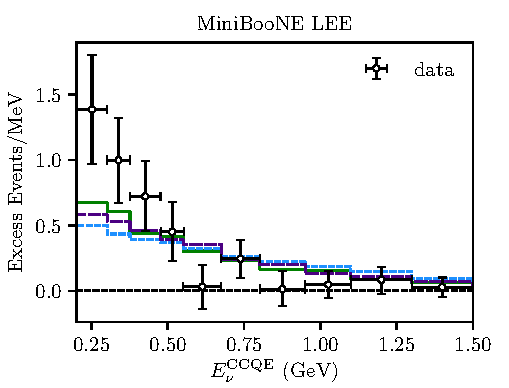
\includegraphics[width=0.49\textwidth]{Enu_reco.pdf}
    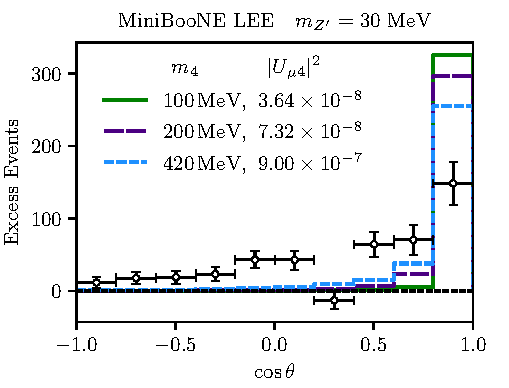
\includegraphics[width=0.49\textwidth]{Theta_reco.pdf}\\
    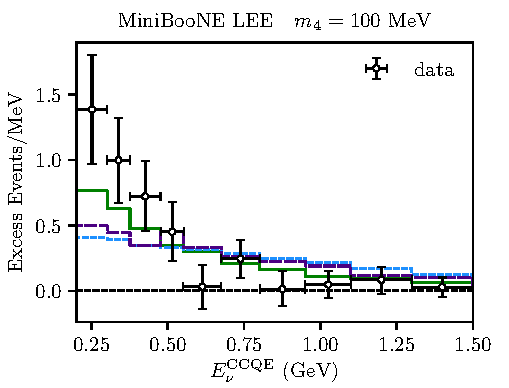
\includegraphics[width=0.49\textwidth]{Enu_reco_m4=100mev.pdf}
    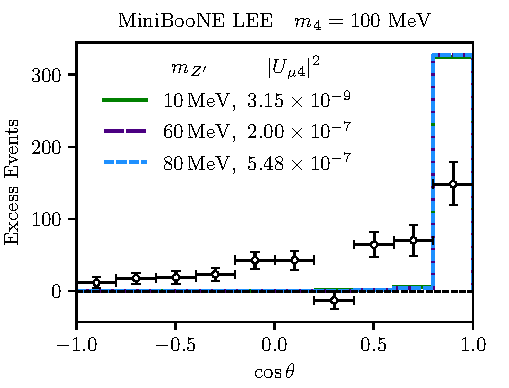
\includegraphics[width=0.49\textwidth]{Theta_reco_m4=100mev.pdf}\\
    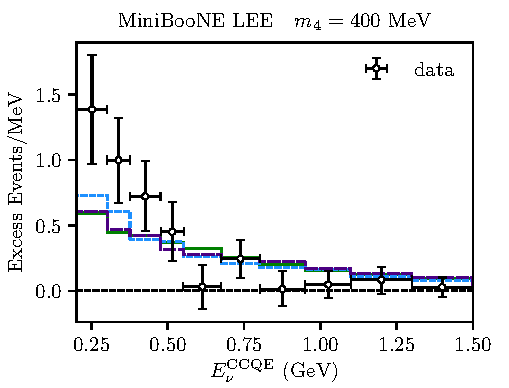
\includegraphics[width=0.49\textwidth]{Enu_reco_m4=400mev.pdf}
    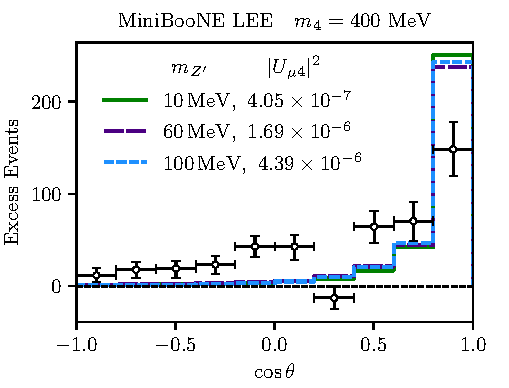
\includegraphics[width=0.49\textwidth]{Theta_reco_m4=400mev.pdf}
    \caption[New physics prediction and data at MiniBooNE.]{Data and new physics prediction for the reconstructed neutrino energy at MiniBooNE under the assumption of CCQE scattering (\textbf{left}), and for the cosine of the angle between the visible EM and the neutrino beam (\textbf{right}). We fix couplings so that the total number of events at MiniBooNE equals 334.~\label{fig:MB_distributions}}
\end{figure}
%

To verify that the new physics signal is important in neutrino-electron studies, we also plot kinematical distributions for the benchmark point (BP) for different detectors. This corresponds to $m_{Z^\prime} = 30$ MeV, $\alpha \epsilon^2 = 2\times10^{-10}$, $\alpha_D = 1/4$, $|U_{\mu 4}|^2 = 9\times10^{-7}$ and $m_4 = 420$ MeV. The interesting variables are the energy asymmetry of the dielectron pair 
\begin{equation}
    |E_{\rm asym}| = \frac{|E_+ - E_-|}{E_+ + E_-},
\end{equation}
as well as the separation angle $\Delta \theta_{e^+e^-}$ between the two electrons. These variables are plotted in Fig.~\ref{fig:other_distributions} at MC truth level, before any smearing or selection takes place. We also plot the total reconstructed energy $E_{\rm vis} = E_{e^+} + E_{e^-}$ and the quantity $E_{\rm vis} \theta^2$, where $\theta$ stands for the angle formed by the reconstructed EM shower and the neutrino beam. $E_{\rm vis}$ and $\theta$ are computed after smearing, but before the selection into overlapping pairs takes place.

%
\begin{figure}[h]
    \centering
    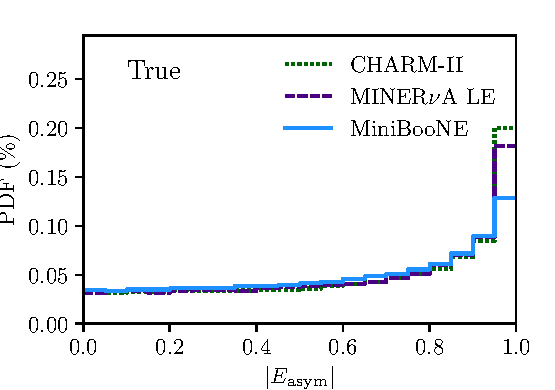
\includegraphics[width=0.49\textwidth]{Easym_v1.pdf}
    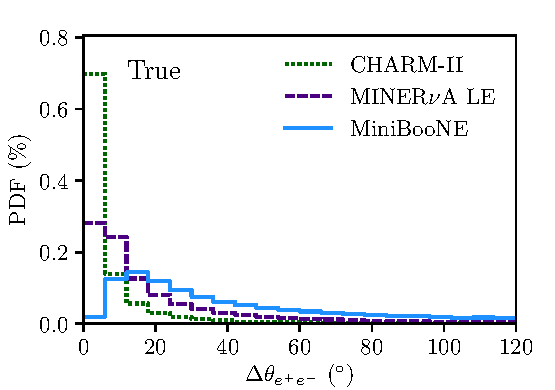
\includegraphics[width=0.49\textwidth]{DeltaTheta_v1.pdf}
    \\
    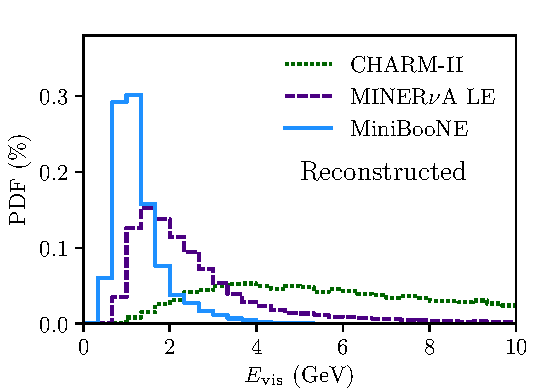
\includegraphics[width=0.49\textwidth]{Evis_v1.pdf}
    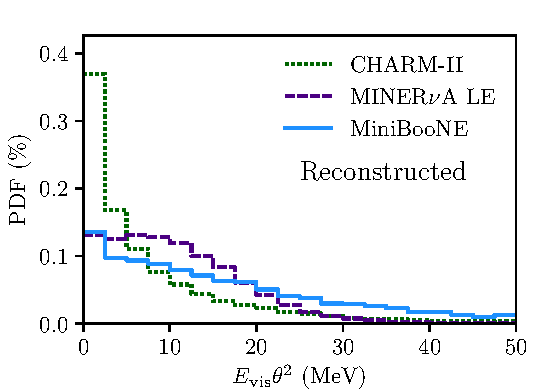
\includegraphics[width=0.49\textwidth]{Etheta2_v1.pdf}
    \caption[Dark neutrino kinematical distributions.]{Kinematical distributions for the new physics events at CHARM-II, MINER$\nu$A LE and MiniBooNE for the BP. We show the energy asymmetry (\textbf{top left}), the electron separation angles (\textbf{top right}), both at MC truth level. We also show reconstructed ({after smearing}) total visible energy $E_{\rm vis}$ (\textbf{bottom left}) and $E_{\rm vis} \theta^2$ (\textbf{bottom right}).\label{fig:other_distributions}}
\end{figure}


  \subsection{MINER$\nu$A and CHARM-II Analyses}
Neutrino-electron scattering measurements predicate their cuts in the following core ideas: no hadronic activity near the interaction vertex, small opening angle from the beam, $E_e \theta^2 \lesssim 2 m_e$, and the requirement that the measured energy deposition, $dE/dx$, be consistent with that of a single electron. For the NP events, when the coherent process dominates and the mass of the $Z^\prime$ is small, the first two conditions are often satisfied. However, the requirement of a single-electron-like energy deposition removes a significant fraction of the new-physics induced events. This presents a challenge, as the NP events are mostly overlapping electron pairs and will potentially be removed by the $dE/dx$ cut.
In order to circumvent this problem, we perform our analysis not at the final-cut level, but at an intermediate one. This is done differently for CHARM-II and MINER$\nu$A: the CHARM-II experiment provides data as a function of $E_e \theta^2$ without the $dE/dx$ cut, and \minerva provides data as a function of the measured $dE/dx$ after analysis cuts on $E_e \theta^2$.

We have developed our own MC simulation for candidate electron pair events in MiniBooNE, MINER$\nu$A and CHARM-II (see the Supplemental Material for more details on detector resolutions, precise signal definition and resulting distributions). We only consider the coherent part of the cross section to avoid hadronic-activity cuts, which is conservative. We also select only events with small energy asymmetries and small opening electron angles.
When required, we assume the mean $dE/dx$ in plastic scintillator to follow the same shape as the NC $\pi^0$ prediction. Our prediction for new physics events for the BP point is show in Fig. \ref{fig:NP_events} on top of the \minerva ME and CHARM-II data and MC prediction. This includes all analysis cuts, which we describe below.   
%We calculate the mean $dE/dx$ in plastic scintillators~\cite{NIST:2018} according to~\cite{Leo:1987kd,Tanabashi:2018oca}. 

The CHARM-II analysis is mostly based on Fig. 1 of~\cite{Vilain:1994qy}. This sample is shown as a function of $E\theta^2$ and does not have any cuts on $dE/dx$. It contains all events with shower energies between $3$ and $24$ GeV, and our final cut on $E\theta^2$ is fixed at $28$ MeV. For \minerva, the event selection is identical for the LE and ME analyses~\cite{Park:2015eqa,Valencia:2019mkf}. The minimum shower energy required is $0.8$ GeV in order to remove the $\pi^0$ background and have reliable angular and energy reconstruction. Events are kept only when they meet the following angular separation criterion: $E_e \theta^2 < 3.2\times 10^{-3}~{\rm ~GeV ~rad^2}$. A final cut is applied, ensuring $dE/dx < 4.5~{\rm MeV} / 1.7~{\rm cm}$. The \minerva analyses use the data outside the previous $dE/dx$ cut to constrain backgrounds. This sideband is defined by all events with $E_e\theta^2 > 5 \times 10^{-3} {\rm ~GeV ~rad^2}$ and $dE/dx < 20~{\rm MeV}/1.7~{\rm cm}$. Using this sideband measurement, the collaboration tunes their backgrounds by ($0.76$, $0.64$, $1.0$) for ($\nu_e$CCQE, $\nu_\mu$NC, $\nu_\mu$CCQE) processes in the LE mode. Our LE analysis uses the data shown in Fig. 3 of~\cite{Park:2015eqa} where all the cuts are applied except for the final $dE/dx$ cut. In our final event selection, we require that the sum of the energy deposited be more than $4.5$ MeV$/ 1.7$ cm, compatible with an $e^+e^-$ pair and yielding an efficiency of $90\%$.

The \minerva ME data contains an excess in the region of large $dE/dx$~\cite{Valencia:2019mkf}, where the NP events would lie. This excess is attributed to NC $\pi^0$ events, and grows with the shower energy. With normalization factors as large as 1.7, the collaboration tunes primarily the NC $\pi^0$ prediction in an energy dependent way. After tuning, the total NC $\pi^0$ sample corresponds to $20\%$ of the total number of events before the $dE/dx$ cut.

To place our limits, we perform a rate-only analysis by means of a $\chi^2$ test statistic (detailed in the Supplemental Material). We incorporate uncertainties in background size and flux normalization as nuisance parameters with Gaussian constraint terms. For the neutrino-electron scattering and BSM signal, we allow the normalization to scale proportionally to the same flux uncertainty parameter. 
The background term also scales with the flux-uncertainty parameter but has an additional nuisance parameter to account for its unknown size. We obtain our constraint as a function of heavy neutrino mass $m_4$, and mixing $|U_{\mu 4}|$ assuming a $\chi^2$ with two degrees of freedom~\cite{Tanabashi:2018oca}.

In our nominal \minerva LE (ME) analysis, we allow for 10\% uncertainty on the flux~\cite{Aliaga:2016oaz}, and 30\% (40\%) uncertainty on the background motivated by the amount of tuning performed on the original backgrounds. Note that the nominal background predictions in the \minerva LE (ME) analysis overpredicts (underpredicts) the data before tuning, and that tuning parameters are measured at the 3\% (5\%) level~\cite{Park:2013dax,Valencia:2019mkf}.
We also perform a background-ignorant analysis in which we assume 100\% uncertainty for the background normalization, which changes our conclusions by only less than a factor of two. This emphasizes the robustness of our \minerva bound, since the NP typically overshoots the low number of events in the sideband. For the benchmark point of~\cite{Bertuzzo:2018itn}, we predict a total signal of 232 (4240) events for \minerva LE (ME).

For CHARM-II, the NP signal lies mostly in a region with small $E\theta^2$. Thus, we constrain backgrounds using the data from $28 < E\theta^2 < 60$ MeV rad$^2$. This sideband measurement constrains the normalization of the backgrounds in the signal region at the level of $3\%$.
The extrapolation of the shape of the background to the signal region introduces the largest uncertainty in our analysis. For this reason, we raise the uncertainty of the background normalization from $3\%$ to a conservative $10 \%$ when setting the limits. Flux uncertainties are assumed to be $4.7\%$ and $5.2\%$ for neutrino and antineutrino mode~\cite{Allaby:1987bb}, respectively, and are applicable to the new-physics signal, $\nu-e$ scattering prediction, and backgrounds. 
Uncertainties in the $\nu-e$ scattering cross sections are expected to be sub-dominant and are neglected in the analysis~\cite{deGouvea:2006hfo}. For CHARM-II, the NP also yields too many events in the signal region, namely $\approx 2.2\times10^{5}$ events for the benchmark point of~\cite{Bertuzzo:2018itn} in antineutrino mode. If we lower $|U_{\mu4}| = 10^{-4}$ and $m_4 = 100$ MeV, CHARM-II would still have $\approx 3 \times 10^3$ new physics events. 

We have performed our own fit to the MiniBooNE energy spectrum using the data release from~\cite{Aguilar-Arevalo:2018gpe}, and our results agree with~\cite{Bertuzzo:2018itn}. The data release, however, only contains information about the neutrino energy and baseline distance. Thus, the re-weighting procedure for the model of interest can only be performed approximately. A proper analysis can be performed only if true and reconstructed electron angles and energies per simulated event are given.  
%
\begin{figure}[h]
    \centering
    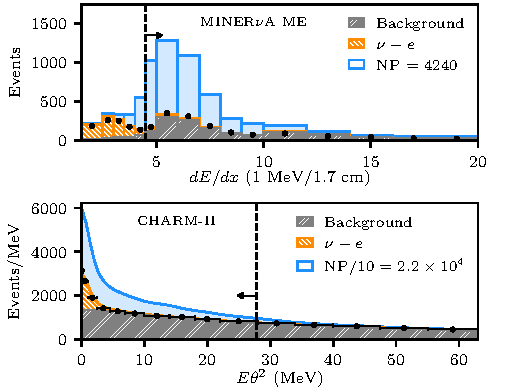
\includegraphics[width=0.75\textwidth]{both_cartoon.pdf}
    \caption[New physics signal in neutrino-electron scattering data.]{Neutrino-electron scattering data in $dE/dx$ at \minerva (top) and in $E\theta^2$ at CHARM-II (bottom). Error bars are too small to be seen. For both experiments, we show the $\nu-e$ signal and total background prediction quoted (after tuning at MINER$\nu$A), as well as the NP prediction (divided by 10 at CHARM-II). The cuts in our analysis our shown as vertical lines. \label{fig:NP_events}}
\end{figure}


%
\begin{figure}[h]
    \centering
    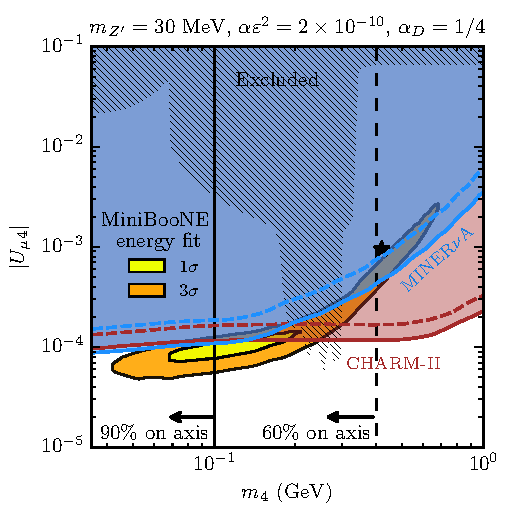
\includegraphics[width=0.7\textwidth]{bounds.pdf}
%     \caption[New constraints on dark neutrinos.]{The MiniBooNE region of interest from~\cite{Bertuzzo:2018itn}, only fitted to the energy distribution, is shown as closed yellow (orange) regions for one (three) sigma C.L. The benchmark point, chosen to provide a good angular distribution fit, is shown as a black star. Exclusion from heavy neutrino searches is shown as a hatched background. Our new constraints at 90\% C.L. using \minerva are shown in blue for our nominal 30\% background normalization uncertainty (solid) and conservative case of 100\% background uncertainty (dashed). Our CHARM-II bound is shown in cherry red, where the 3\% background normalization from the sideband is shown as a solid curve and the conservative 10\% case as a dashed curve. The solid vertical black line at 100 MeV signals the point where 90\% of NP events lie in the most forward bin in the MiniBooNE angular distribution, and the dashed one where 60\% of events do so. Other relevant assumed parameters are shown above the plot; changing them does not change our conclusion.}
    \caption[New constraints on dark neutrinos.]{The fit to the MiniBooNE energy distribution from~\cite{Bertuzzo:2018itn} is shown as closed yellow (orange) region for one (three) sigma C.L., together with the benchmark point (${\bf\odot}$). Our constraints are shown at 90\% C.L. for \minerva LE in blue (solid -- 30\% background normalization uncertainty, dashed -- conservative 100\% case), for \minerva ME in cyan (solid -- 40\% background normalization uncertainty, dashed -- conservative 100\% case), and for CHARM-II in red (solid -- 3\% background normalization from the sideband constraint, dashed -- conservative 10\% case). Vertical lines show the percentage of excess events at MiniBooNE that lie in the most forward angular bin. Exclusion from heavy neutrino searches is shown as a hatched background. Other relevant assumed parameters are shown above the plot; changing them does not alter our conclusion.\label{fig:final_plot}}
\end{figure}
%

\section{Results and Prospects}
The resulting limits on dark neutrinos in neutrino-electron scattering experiments are shown in the $|U_{\mu 4}|$ vs $m_4$ plane at 90\% confidence level (CL) in~\reffig{fig:final_plot}. The MiniBooNE fit from~\cite{Bertuzzo:2018itn} is shown, together with vertical lines indicating the percentage of events at MiniBooNE that populate the most forward angular bin.
We have chosen the same values of $\varepsilon$, $\alpha_D$, and $m_{Z^\prime}$ as used in~\cite{Bertuzzo:2018itn}, and shown their benchmark point ($m_4 = 420$ MeV and $|U_{\mu 4}|^2 = 9 \times 10^{-7}$) as a dotted circle. For these parameters, we can conclude that a good angular distribution at MiniBooNE is in large tension with neutrino-electron scattering data.
We note that the MiniBooNE event rate scales identically to our signal rate in all the couplings, and the dependence on $m_{Z^\prime}$ is subleading due to the typical momentum transfer to the nucleus, provided $m_{Z^\prime} \lesssim 100$ MeV .
This implies that changing the values of these parameters does not modify the overall conclusions of our work. In addition, for this realization of the model, larger $m_{Z^\prime}$ implies larger values of $m_4$, increasing the tension between the MiniBooNE fit and our bounds.
Our results from \minerva and CHARM-II are mutually reinforcing given that 
they impose similar constraints for $m_4 \lesssim 200 $ MeV. For larger masses, the kinematics of the signal becomes less forward and the production thresholds start being important. This explains the upturns visible in our bounds, where we observe it first in \minerva and later in CHARM-II as we increase $m_4$, since CHARM-II has higher beam energy. Finally, we emphasize that our analysis can be adapted to other models, such as the dark neutrino realisation of~\cite{Ballett:2018ynz} and scenarios with heavy neutrinos with dipole interactions~\cite{Magill:2018jla}. For the former, however, we do not expect our bounds to constrain the region of parameter space where the MiniBooNE explanation is viable, since most of the signal at MiniBooNE contains hadronic activity which would be visible at \minerva and CHARM-II.

In the near future, our new analysis strategy could be used in the up-coming \minerva ME results on antineutrino-electron scattering. The NP cross section, being the same for neutrino and antineutrinos, is thus more prominent on top of backgrounds.
This class of analyses will also greatly benefit from improved calculations and measurements of coherent $\pi^0$ production and single-photon emitting processes. This is particularly important given the excess seen in the \minerva ME analysis.
A complementary result can also be obtained by neutrino-electron scattering measurements at NO$\nu$A, which will sample a different kinematic regime as its off-axis beam peaks at lower energies and expects fewer NC~$\pi^0$ events per ton.
Beyond neutrino-electron scattering, the BSM signatures we consider could be lurking in current measurements of $\pi^0$ production, \textit{e.g.}, at MINOS~\cite{Adamson:2016hyz} and MINER$\nu$A~\cite{Wolcott:2016hws}~\footnote{This $\nu_e$CCQE measurement by \minerva observes a significant excess of single photon-like showers attributed to diffractive $\pi^0$ events. These are abundant in similar realizations of this NP model~\cite{Ballett:2018ynz}.}, and in analyses like the single photon search performed by T2K~\cite{Abe:2019cer}.
To summarize, a variety of measurements are underway to further lay siege to this explanation of the MiniBooNE observation and, simultaneously, start probing testable neutrino mass generation models, as well as other similar NP signatures. It is clear that understanding neutrino cross sections will be crucial as we move forward.
